\chapter{Query Processing}
\label{chap:Query Processing}
So far, we have studied base techniques that improve OLAP\todo{rephares} performance for in-memory, read-only databases. However, a high-performance \bd~application does not only rely on using the correct data format, compression, indexes, parallelization, and implementation. In this chapter we elaborate query processing techniques.

In Section \ref{sub:Business Discovery, Queries, and SQL}, we explained how \bd~applications relate to traditional queries. We saw that a \bd~application must support listing of rows, filtering, joining, and grouping/aggregation. In this chapter, we focus on query processing, mainly joining, grouping and aggregation, and query optimization.


%storing the data in the correct format, using light-weight compression algorithms, and index and other structures to aid performance. We show that algorithms and optimizations done when processing queries are also important.

%Grouping and Aggregation are the single most important functionality for a \bi~applications, as people require data summary and not data details. Joining is key for these applications, and perhaps even more for \bd~systems, since a filter in one table must quickly propagate to the other tables.

%As mentioned in the background section lthough a \bd~system does not need to support SQL, we still need traditional query techniques, like joining, grouping and aggregation.

\newpage

\section{Joining}
\label{sec:Joining}
Joining is a common database operation that combines records from two or more tables. In our research, we have studied several DBMSes, and seen how their join algorithms work. As we saw in Section \ref{sub:Business Discovery, Queries, and SQL}, joining is also needed for a \bd~application such that interaction with one table can affect the selection, filters, or aggregations in other tables.

For joining two tables, three main methods exist \cite{Bratbergsengen2015-ed}: 
\begin{itemize}
  \item \textit{Partition-based approach}, where records of both tables are split into groups based on the hash value of the keys. This technique is most effective on data volumes that are too large to fit in main memory.
  \item \textit{Sort-merge approach}, where both tables are sorted and then merge results by concatenating records with equal key values. This approach is most effective when one or both operands are sorted in advance.
  \item \textit{Nested loop approach}, which compares all rows in both tables.
\end{itemize}

We find the \textit{nested loop} approach to be the most popular joining algorithm for in-memory and parallel databases \cite{Boncz2002-yj}. The rest of Section \ref{sec:Joining} will therefore only discuss this method.

\subsection{Nested Loop Algorithms}
\label{sub:Nested Loop Algorithms}

% Basic nested join functionality
In its simplest form, the \textit{nested loop} method compares all the join keys \todo{all?} in all rows directly using a double loop. This simple algorithm has a runtime of $O(n*m)$ where $n$ and $m$ is the size of tables A and B respectively. However, to improve performance in a \textit{nested loop} algorithm, hashmaps are commonly used. Usually, the join is performed by hashing the smaller (inner) relation first, then probe the hashmap by scanning the larger (outer) relation. 

In a star or snowflake schema, dimension tables are usually considered as the inner relations \cite{Barber2012-xt, Raman2013-em}. In other words, the keys of these tables will be used to create the hashmaps in the join. In the second phase of the algorithm, the fact table will probe the generated hashmaps to complete the join. 

\ffigure{img/nested-loop.png}{An example nested loop join structure. Records are first tested against a Bloom filter. If found in the filter, the join key is searched in the join structure. Records are first hashed, and then each entry in the hash table is the root of a binary tree. Courtesy of \cite{Bratbergsengen2015-ed}.}{fig:nested-loop}

Bratbergsengen \ea~show how a combination of hash tables, bloom filters, and binary trees can be used in a \textit{nested join} algorithm. In the probe phase, keys are first checked towards a Bloom filter (Section \ref{sub:Bloom Filter}). Bloom filters never return false negatives and is an efficient way of reducing the numbers of keys entering the join. If the key is found in the Bloom filter lookup, it is hashed and checked up against a hybrid hashmap/binary-tree structure. In this structure, each entry in the hashmap is the root node of a binary tree which are used to efficiently look up values. The join algorithm is illustrated in Figure \ref{fig:nested-loop}.

% Modifications
In the nested loop approach, one of the operands might be partitioned \cite{Bratbergsengen2015-ed}. For example, a join might be partitioned by only hashing a subset of the inner relation at a time. The entire join algorithm will then include several probe passes over the outer relation, one for each subset. Historically, this technique has been applied to ensure the whole hash structure fits in RAM. We conclude that a similar concept can be applied to CPU caches and that the join algorithm might benefit from partitioning the inner relation such that each subset fits in the CPU cache.

We see that several DBMSes in this research use a \textit{nested loop} join variant with Bloom filters, including \oracle~\cite{Lahiri2015-mz}, \ibm~\cite{Raman2013-em} and \blink~\cite{Raman2008-gi}. Barber \ea~explains how Bloom filters are effective in eliminating non-matching join outers before they enter the join \cite{Barber2014-ey}.

Our research has shown that one of the key design goals for efficient joining using the \textit{nested loop} approach with hashmaps, is to keep the hash tables collision free \cite{Raman2008-gi, Raman2013-em}. One way to ensure this is to use the dictionary keys in \de~as a perfect hashing function. If a table is joined on several keys, a minimal perfect hash can be calculated.

Regarding implementation, it is important that the algorithm and the hash table are \textit{cache-aware}. One way to improve cache performance in a \textit{nested loop} join, is to use linear probing instead of open-chain addressing for the hashmap \cite{Raman2008-gi}. Open-chain addressing should only be used for overflow buckets.

Joining should be done in parallel for ultimate performance. For instance, the hash tables can be built using multiple threads \cite{Barber2014-ey}. We see that some \textit{nested loop} based algorithms partition the input to improve cache performance. However, this decision might as well be a parallelization decision \cite{Neumann2011-uq}. A system studied in our research that employs high-performance parallel joining is \ibm \cite{Raman2013-em}.

\subsection{Invisible Join}
\label{sub:Invisible Join}

\begin{figure}
  \centering
  \begin{subfigure}{0.48\textwidth}
    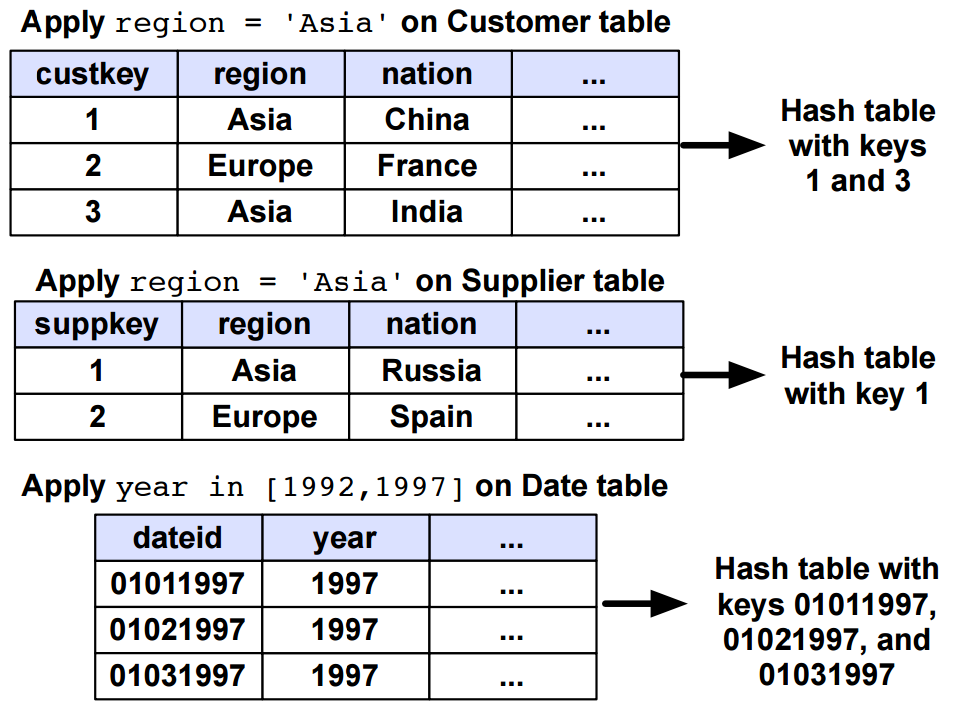
\includegraphics[width=\textwidth]{img/invisible-join-1.png}
    \caption{The first phase of the \textit{invisible join}. Predicates are evaluated on every dimension table, and matching rows are put into a hash table.}
    \label{fig:invisible-join-1} 
  \end{subfigure}
  \begin{subfigure}{0.48\textwidth}
    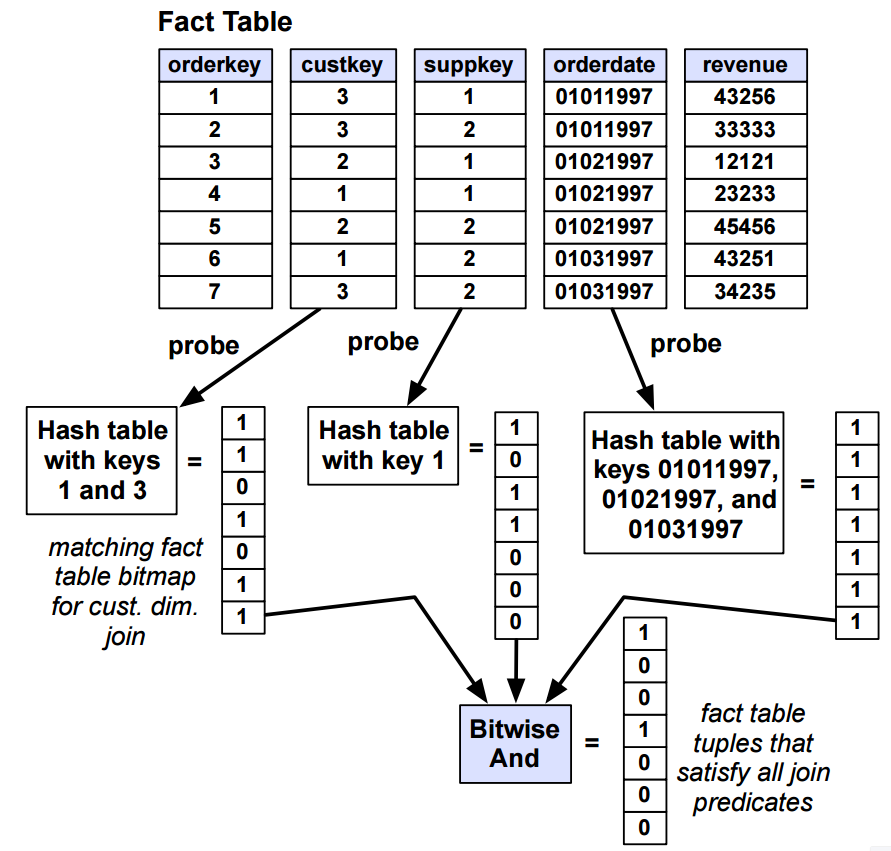
\includegraphics[width=\textwidth]{img/invisible-join-2.png}
    \caption{The second phase of the \textit{invisible join}. The fact table is scanned and probed towards the hash tables generated in in the previous step. Each relation generates a bitmap which is combined using a bitwise \texttt{AND} operation.}
    \label{fig:invisible-join-2} 
  \end{subfigure}
  \begin{subfigure}{0.48\textwidth}
    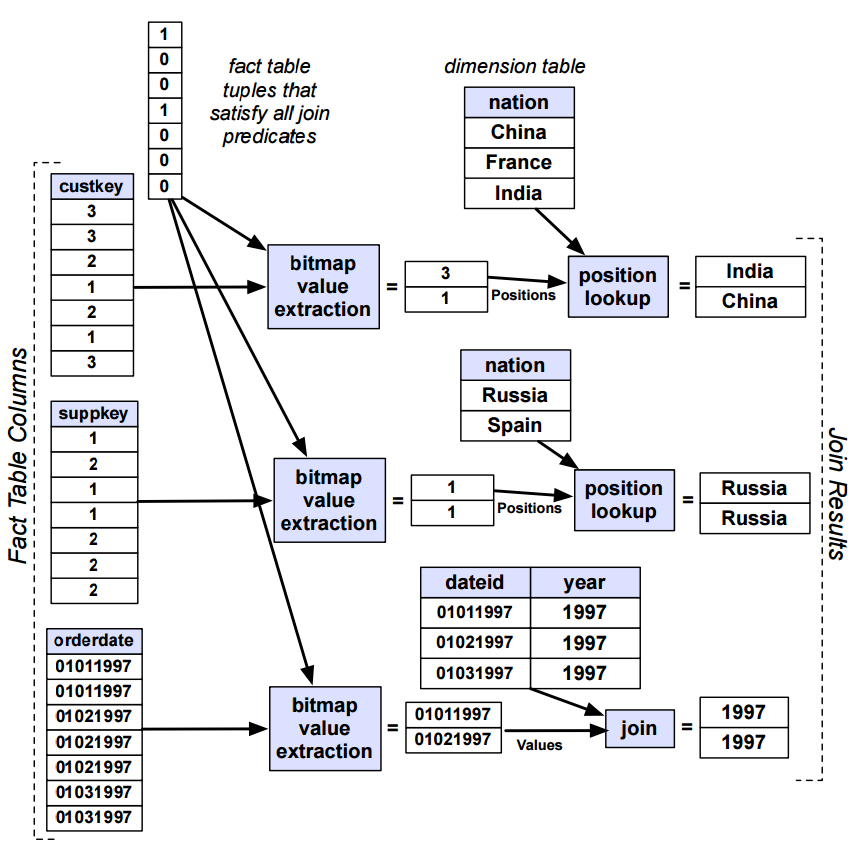
\includegraphics[width=\textwidth]{img/invisible-join-3.png}
    \caption{The third phase of the \textit{invisible join}. The foreign keys for the join columns are extracted from the fact table. The extracted values use the  hash tables from the firt phase to complete the join.}
    \label{fig:invisible-join-3} 
  \end{subfigure}
  \caption{The \textit{invisible join} algorithm from Abadi \ea~Courtesy of \cite{Abadi2008-dd}.}
  \label{fig:invisible-join} 
\end{figure}

Our research has identified several different join implementations that are suited for OLAP workloads and in-memory processing. In this section, we will focus on one such implementation, namely Abadi \ea's \textit{invisible join} \cite{Abadi2008-dd}. The reason we have chosen to elaborate on this algorithm is two-fold. First, the algorithm is well explained by Abadi \ea, and the paper contains detailed figures that help the understanding of how the algorithm works. Secondly, the algorithm uses some temporary data structures (bitmaps and hash tables) which we believe might be relevant structures for indexing or caching.

The \textit{invisible join} algorithm assumes a star schema style table, and works by rewriting joins into predicates on the foreign keys in the fact table. To improve cache performance, the algorithm minimizes the values that need to be extracted out of order, and to reduce memory traffic, it avoids unnecessary materialization steps. 

The \textit{invisible join} algorithm works in three phases:
\begin{enumerate}
  \item The smaller relations (dimension tables) are hashed, but if the tables are filtered with predicates, only matching keys are inserted into the hash table.
  \item Per hashmap generated in the first phase of the algorithm, the larger relation is probed, and a bitmap indicating qualifying is created. The resulting bitmap for each dimension table is combined using bitwise operations, like \texttt{AND} or \texttt{OR}. Creating these bitmaps might also happen in parallel. 
  \item To complete the join, keys in the foreign columns in the fact table are extracted using the bitmap from the previous step. In this step, either positional lookup (for sorted values) or the hash tables from the first step can be used to get the projected values.
\end{enumerate}
The entire algorithm is illustrated in Figure \ref{fig:invisible-join}.

We gave the \textit{invisible join} as an example join algorithm, because we believe a similar method is needed in a \bd~application with multiple tables. We see that hash tables from the first phase and bitmaps from the second phase are candidates for caching, a technique we saw in Section \ref{sec:Caching and Dynamic Index Generation} commonly used to improve read performance.

\section{Grouping and Aggregation}
\label{sec:Grouping and Aggregation}
The ability to group and aggregate data is perhaps one of the most important capabilities for \bi~and \bd~applications. In Section \ref{sub:Business Discovery, Queries, and SQL} we saw that users are interested in reports that can be analyzed quickly, which means the summarization and categorization of data.

Conceptually, grouping and aggregation are relatively straightforward: The record set is scanned and divided into groups based on one or more attributes, and for each cluster an accumulator is held \cite{Bratbergsengen2015-ed}. Accumulators can be of various types, which includes \term{count}, \term{min}, \term{max}, \term{average}, and \term{sum}. Some aggregates require just a single memory cell, like \term{count} and \term{sum}, others are more involved and require more memory to calculate. A suitable structure stores the aggregated results, as a hash table or linear array. 

Our research has shown that multiple optimizations can be done to improve grouping and aggregation performance. For instance, grouping and aggregation can be performed at the same time as the data is scanned and filtered \cite{Lemke2010-is}. This is done in \blink, where the core idea is a generalized scan that filters, groups, and aggregates on a single scan over the data \cite{Raman2008-gi}.

Dictionary encoding can simplify grouping and aggregation, since dictionary entries can be used as a perfect hash for directly storing the aggregated results \cite{Boncz2005-wj, Lemke2010-is}. Such optimization is done in \monetx~and \blink. Besides, some aggregation operations do not need to scan the entire column, as it is sufficient to use the values in the dictionary. For instance, the maximum value in a column's dictionary will also be the maximum value for that column.


\ffigure{img/vector-group-by}{The \term{Vector Group By} technique used in \oracle. Courtesy of \cite{Oracle2015-fs}.}{fig:vector-group-by}

For composite \texttt{GROUP BY} operations, a multidimensional structure may be used. \oracle~uses a technique that they call \term{Vector Group By}, which is an algorithm that uses a compact multidimensional array for storing aggregate results \cite{Oracle2015-fs}. The \term{Vector Group By} algorithm works as following:
\begin{enumerate}
  \item The query scans the dimension tables.
  \item A key vector is created per table based on the results in the previous step. The key vectors are used to filter the fact table when predicates are applied to the foreign tables. They work like Bloom filters, except they do not return false negatives.
  \item An in-memory accumulator is created based on the key vectors which are used to store the accumulated results.
  \item The fact table is scanned, and data is accumulated in the structure established in the previous step. If there is a key vector that does not contain the foreign key, the row is should not be a part of the aggregation.
\end{enumerate}

Figure~\ref{fig:vector-group-by} illustrates the \term{Vector Group By} algorithm.

\ffigure{img/parallel-group-by}{Simple illustration of parallel grouping and aggregation in \ibm. Several threads perform the operations using a local hash table. In the second phase of the algorithms, threads are assigned a partition of the hash space and merge all local hash tables into a global partitioned hash table. Courtesy of \cite{Raman2013-em}.}{fig:parallel-group-by}

Grouping and aggregation should be done in parallel for ultimate performance. In \ibm, multiple threads perform local grouping on local hash tables on column partitions \cite{Raman2013-em}. In the second phase of this algorithm, each thread picks a partition of the local hash tables using a global counter and merges the local tables into a global partitioned hash table. The process is illustrated in Figure \ref{fig:parallel-group-by}.


\section{Query Optimization}
\label{sec:Query Optimization}
Query optimization is a large field within computer science and databases and was initially thought to be left out of this research. However, several systems identified in our literature survey have included some sort of query optimization. We will, therefore, briefly discuss this topic in this section. 

Query optimizers should try to reduce the search space \cite{Boncz2002-yj, Stonebraker2005-qz}. Search space is reduced in \blink, where the only operation to access a table is via scans, and joining and grouping is done in a prespecified order \cite{Barber2012-xt}. Besides, query performance is increased if data is filtered out as early as possible in the plan \cite{Lamb2012-kg}. For instance, the most selective tables in a join operation should be joined first \cite{Holloway2008-rr}.

If compression is applied to the database, it is important that the query optimizer is aware of this \cite{Westmann2000-mz}. It must take into account that the compressed columns can be worked on directly without decompression \cite{Stonebraker2005-qz}.

In a distributed environment, the query optimizer should minimize the need for coordination by assigning query operations that can run independently on each machine \cite{Exasol2014-xh}. 

We conclude this section by saying that the query optimizer must utilize possible optimizations allowed by the design. This includes:
\begin{itemize}
  \item Database statistics (Section \ref{sec:Database Statistics}) can be used to skip blocks if columns are horizontally partitioned.
  \item Dictionary keys for a partition can be checked before scanning a column. If a key is not present in the dictionary, the partition can be skipped.
  \item Complicated predicates can be turned into \texttt{IN} predicates based on entries in the dictionary.
\end{itemize}

\section{Querying Directly on Compressed Data}
\label{sec:Querying Directly on Compressed Data}
We find one of the most important technique for good query performance to operate directly on compressed data, which we have studied in Section \ref{sub:Working Directly on Compressed Data}. As we have seen, this is especially important when using dictionary compression, such simple integer operations can evaluate most predicates \cite{Abadi2008-dd}. If the data is bitpacked, queries can be processed in a SIMD-like fashion, a technique we study in more detail in Section \ref{sec:SIMD}.

Systems querying direcly on compressed data include \cstore~\cite{Stonebraker2005-qz}, \ibm~\cite{Raman2013-em}, \mssql~\cite{Larson2013-mc}, \blink~\cite{Johnson2008-cp}, \sapnw~\cite{Lemke2010-is}. All of these systems claim one of their main benefits in terms of performance is their ability to work directly on the compressed data.

\section{Measure and Dimension Attributes}
\label{sec:Measure and Dimension Attributes}
We see that some systems make a distinction between measure and dimension attributes \cite{Johnson2008-cp, Kamkolkar2015-iq}. A dimension attribute typically answers questions like "where", "what", and "when", whereas a measure attribute normally answers in terms of "how much" \cite{noauthor_undated-es}. 

We have no specific evidence of what this classification can do to aid query processing, but we believe it can help determine which results that should be cached. For dimension attributes, join indexes and hash tables used for joining and grouping are candidates for caching. For measure attributes, aggregations and query results can be cached.

We also believe the distinction between the two types of attributes can be used for data placement. In a banked layout, used in \blink, or in column projections, used in \cstore, dimension attributes will benefit from being in the same data bank or column projection to improve join performance.

\section{Chapter Conclusion}
\label{sec:Chapter Conclusion}
In this chapter, we have seen that \bd~applications require joins to associate several tables in an application. We reccomend a \textit{nested loop} algorithm for this, because this is the most popular joining algorithm for in-memory and parallel databases. The join could be inspired by Abadi \ea's \textit{invisible join}. In addition, partitioning the inner relation and using Bloom filters should be considered.

We have seen that grouping and aggregation is perhaps the most important capabilities for a \bd~application. Suitable structures should be used.

\todo{Finish this conclusion}

%We conclude this chapter that join should be executed using a \term{nested loop} algorithm. This type of algorithm is suited for joins where tables fit in memory, which we assume. We also recommend adding Bloom filters to the structures to limit the number of keys entering the join. We recommend using a technique similar to Abadi \ea's \algmet{Invisible Join} for joining.

%We also encourage investigating the benefits of caching temporary structures used in both cache and aggregation. In the case of \algmet{Invisible Join}, the predicate bitmaps can be cached.

%Queries must also work directly on compressed data, as concluded in Chapter \ref{chp:Compression}.
